\documentclass{article}
\usepackage{amsmath,amssymb,amsthm}
\usepackage{enumerate}
\usepackage{mathtools}
\usepackage{graphicx}
\usepackage{caption}
\usepackage{bm}
\newcommand{\solution}{\noindent \textbf{Solution: }}
\newtheorem{theorem}{Theorem}
\newtheorem{question}[theorem]{Question}
\newtheorem{answer}[theorem]{Solution}
\newcommand{\myvec}[1]{\ensuremath{\begin{pmatrix}#1\end{pmatrix}}}
\newcommand{\norm}[1]{\left\lVert#1\right\rVert}
\let\vec\mathbf
\begin{document}
\begin{question}
	Show that the unit direction vector inclined equally to the coordinate axes is $\myvec{\frac{1}{\sqrt{3}} \\ \frac{1}{\sqrt{3}} \\ \frac{1}{\sqrt{3}}}$.
\end{question}
\solution Let $\vec{m}$ be the given unit vector such that $\vec{m}$ = $\myvec{m_x \\ m_y \\ m_z}$.Let $\vec{e}_1=\myvec{1 \\ 0 \\ 0}$, $\vec{e}_2=\myvec{0 \\ 1 \\ 0}$ and $\vec{e}_3=\myvec{0 \\ 0 \\ 1}$ be the direction vectors of the coordinate axes.
As $\vec{m}$ is a unit vector, so $\norm{\vec{m}} =1$ and also we are given is that $\vec{m}$ is inclined equally to the coordinate axis, 
\begin{equation}
\vec{e}_1^T\vec{m} =\vec{e}_2^T\vec{m}=\vec{e}_3^T\vec{m}
\end{equation}
Now, $(1)$ implies 
\begin{align*}
	(\vec{e}_1 -\vec{e}_2)^T\vec{m} = 0 \\
	(\vec{e}_2 -\vec{e}_3)^T\vec{m} = 0 \\
	(\vec{e}_3 -\vec{e}_1)^T\vec{m} = 0
\end{align*}
Thus, converting above system of equations into matrix form, we get
\begin{align}
& \myvec{+1 \quad  -1 \quad +0 \\ +0 \quad +1 \quad -1 \\ -1 \quad +0 \quad +1 }\myvec{m_x \\ m_y \\ m_z} = \myvec{0 \\ 0 \\ 0}  \xRightarrow[R_1+R_3]{R_3=} \\
& \myvec{+1 \quad  -1 \quad +0 \\ +0 \quad +1 \quad -1 \\ +0 \quad -1 \quad +1 }\myvec{m_x \\ m_y \\ m_z} = \myvec{0 \\ 0 \\ 0} 
\xRightarrow[R_2+R_3]{R_3=} \\
& \myvec{+1 \quad  -1 \quad +0 \\ +0 \quad +1 \quad -1 \\ +0 \quad +0 \quad +0 }\myvec{m_x \\ m_y \\ m_z} = \myvec{0 \\ 0 \\ 0} 
\xRightarrow[R_1+R_2]{R_1=} \\
& \myvec{+1 \quad  +0 \quad +1 \\ +0 \quad +1 \quad -1 \\ +0 \quad +0 \quad +0 }\myvec{m_x \\ m_y \\ m_z} = \myvec{0 \\ 0 \\ 0}
\end{align}
From($5$) we find out that
\begin{equation*}
m_x = m_y = m_z
\end{equation*}
Taking, $m_x = m_y = m_z =1$, we get
\begin{equation*}
\vec{m} = \myvec{1 \\ 1 \\1}
\end{equation*}
Also, we know that $\norm{\vec{m}}=1$ as $\vec{m}$ is a unit vector, thus
\begin{equation*}
\vec{m} = \myvec{\frac{1}{\sqrt{3}} \\ \frac{1}{\sqrt{3}} \\ \frac{1}{\sqrt{3}}}
\end{equation*}
Thus, we see that  $\vec{m}$ = $\myvec{ \frac{1}{\sqrt{3}} \\ \frac{1}{\sqrt{3}} \\ \frac{1}{\sqrt{3}}}$ is the unit direction vector inclined equally to the coordinate axes.\\
\begin{figure}[!htb]
	
	\centering
	
	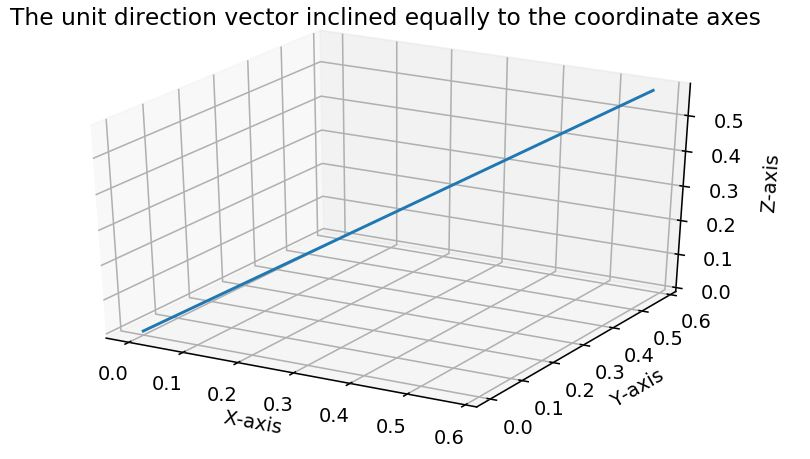
\includegraphics[width=\columnwidth]{assignment1figure.jpg}
	
	\caption{\label{fig1}}
	
	\label{fig:}
	
\end{figure}

\end{document}